

\documentclass{article}
% maths
\usepackage{amsmath}
\usepackage{amssymb}

% figures
\usepackage{graphicx,url}
\usepackage{caption}
\usepackage{subcaption}
\usepackage{float}

%algos
\usepackage{algorithmic}
\usepackage[ruled,vlined]{algorithm2e}
\newcommand{\newalgoline}{\vspace{0.3cm}}
\newcommand{\ttcp}[1]{\tcp{{\footnotesize #1}}}
\newcommand{\fontsizealgo}{\footnotesize}

\newcommand{\nbtx}{nb_{tx}}
\newcommand{\nbrx}{nb_{ack}}
\newcommand{\threshold}{\mathcal{T}}
\newcommand{\blacklist}{blacklist}
\newcommand{\PDRth}{PDR_{th}}



%custom commands
\newcommand{\TODO}[1]{\textcolor{red}{#1}}
\newcommand{\grgs}[1]{\textcolor{red}{[Georgios] #1}}
\newcommand{\vsls}[1]{\textcolor{cyan}{[Vasilis] #1}}
\newcommand{\ft}[1]{\textcolor{blue}{[Fab] #1}}
\newcommand{\red}[1]{\textcolor{red}{#1}}

\usepackage[utf8]{inputenc}
\begin{document}

\section{Evaluation}
\subsection{Reliability}

\begin{figure}
\centering
	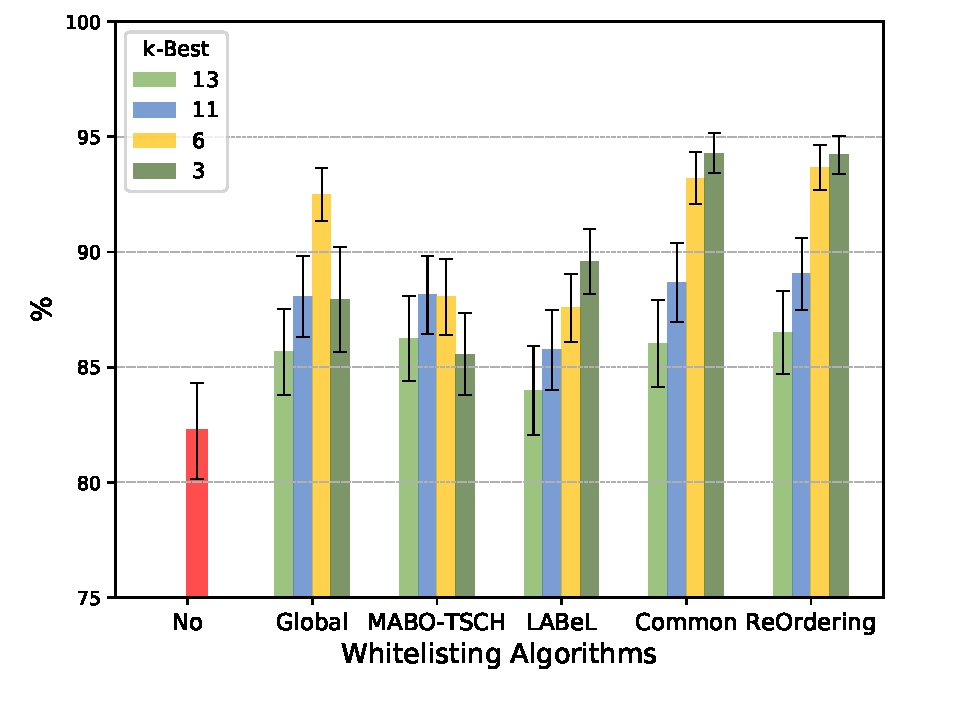
\includegraphics[width=0.99\linewidth]{graphs/PRR}
	\caption{Link-level Packet Delivery Ratio}
	\label{fig:PRR}
\end{figure}

\begin{figure}
\centering
	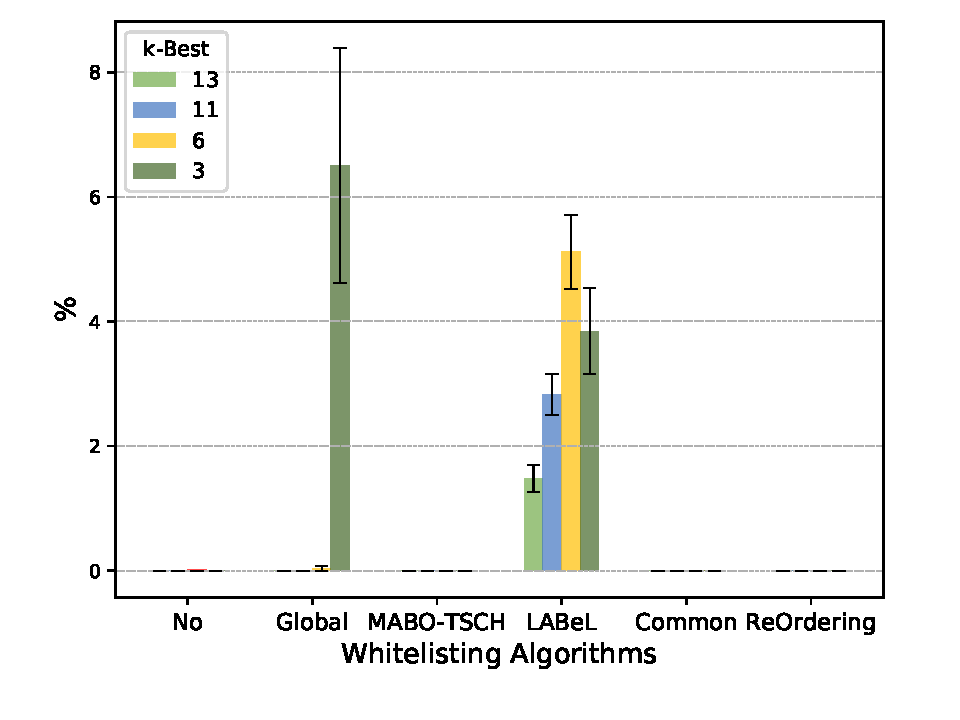
\includegraphics[width=0.99\linewidth]{graphs/collisions}
	\caption{Percentage of Collisions due to parallel transmissions}
	\label{fig:collisions}
\end{figure}


\begin{figure}
\centering
	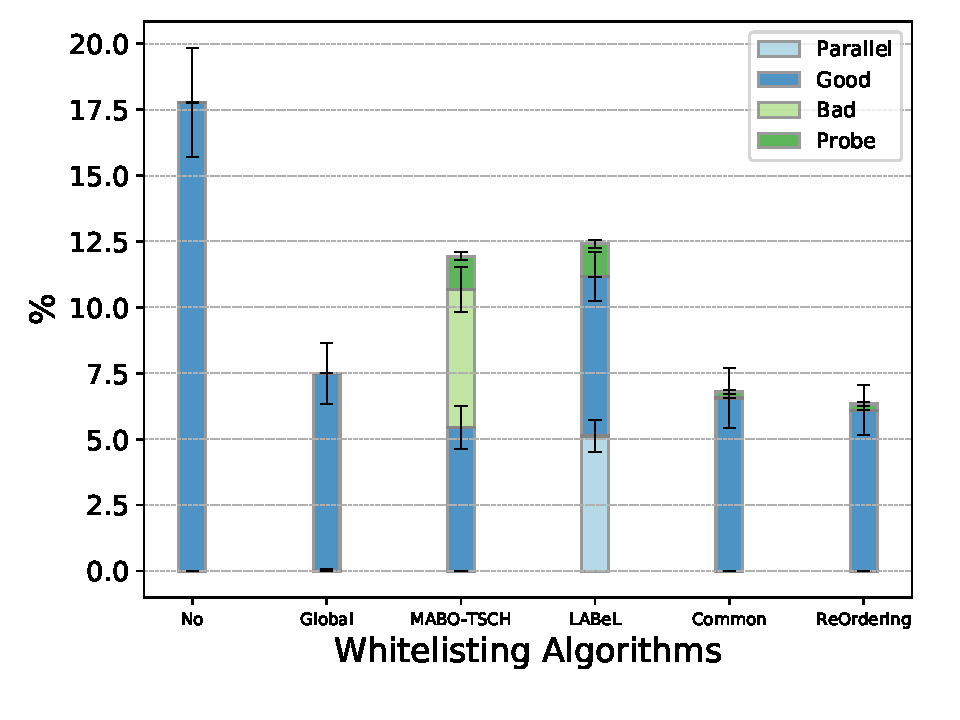
\includegraphics[width=0.99\linewidth]{graphs/collisions_type_10}
	\caption{Classification of the packet drops, in ratio of the total number of data packet generated in the network (whitelist size of 6 radio channels)}
	\label{fig:drop_type}
\end{figure}


\section{Formalization of Internal Collisions}
% New Commands
\newcommand{\SFlength}{\mathcal{S}}
\newcommand{\WhiteLstLengthA}{\mathcal{W}_1}
\newcommand{\WhiteLstLengthB}{\mathcal{W}_2}
\newcommand{\timeslot}{ts}
\newcommand{\positionA}{p_1}
\newcommand{\positionB}{p_2}
\newcommand{\chOffsetA}{ch_1}
\newcommand{\chOffsetB}{ch_2}
\newcommand{\LCM}{f}


Let us calculate the sequence of ASNs where  internal collisions  occur for the example of  Fig.~\ref{fig:offsets-coll}. Let us assume that the whitelists length  of radio links (A,B) and (C,D) are $\WhiteLstLengthA$ and $\WhiteLstLengthB$ respectively. A collision can occur for the physical whitelisted channels in common. In our case, the two whitelists have a common physical channel (2) at positions $\positionA,\positionB$.
In order to have an internal collision should be hold  $\chOffsetA -\chOffsetB = \positionA -\positionB$ where $\chOffsetA,\chOffsetB$ are the channel offsets that have been assigned to the links.
A collision occurs iif the eq.~\ref{eq:freq_hop} hold the following result for the links (A,B) and (C,D) :

%In addition the two lists have a common physical channel in the positions 2 respectively.

\begin{eqnarray} 
	(ASN+\chOffsetA)\pmod{\WhiteLstLengthA}=\positionA  \wedge  (ASN+\chOffsetB)\pmod{\WhiteLstLengthB}=\positionB \\
	\Leftrightarrow  \forall(x,y) \in \mathbb{Z},  ASN+\chOffsetA =\WhiteLstLengthA x+\positionA \wedge ASN +\chOffsetB =\WhiteLstLengthB y+\positionB  \label{eq:eqB} \\ 
   \Leftrightarrow  \WhiteLstLengthA x-\WhiteLstLengthB y=0 \label{eq:eqA}
\end{eqnarray}

The equation~\ref{eq:eqA} is a linear Diophantine equation  of the general form of $ ax+by=c \quad x,y \in \mathbb{Z}$ that has typically an infinite number of  solutions iif the greatest common divisor (GCD) of $a$ and $b$ divides $c$ $(c \mid GCD(a,b))$. Moreover, if $(x_o, y_o)$ is a solution, then the other solutions have the following form:  
\begin{equation}
	x=x_{o}+\frac{b}{d}n  ,\quad 
    y=y_{o}-\frac{a}{d}n \quad n \in \mathbb{Z}
    \label{eq:infinite}
 \end{equation}
\begin{align*}
		\text{where:}\quad \\
        d&=GCD(a,b)
\end{align*}


% wiki reference
Consequently, eq. ~\ref{eq:eqA} has infinite solutions since $d=GCD(\WhiteLstLengthA,\WhiteLstLengthB)$ divides $0$. 
if $\LCM=LCM(\WhiteLstLengthA,\WhiteLstLengthB)$ (Least Common Multiple) then we have a solution  $x_o=\frac{\LCM}{\WhiteLstLengthA}, y_o=\frac{\LCM}{\WhiteLstLengthB}$. All integer solutions are according to eq. ~\ref{eq:infinite} :
\begin{eqnarray}
x=\frac{\LCM}{\WhiteLstLengthA} -\frac{\WhiteLstLengthB}{d}n , \quad 
y=\frac{\LCM}{\WhiteLstLengthB} -\frac{\WhiteLstLengthA}{d}n \quad n \in \mathbb{Z}
\end{eqnarray}
We substitute $x$ in eq. ~\ref{eq:eqB} and we use the equality $\WhiteLstLengthA \cdot \WhiteLstLengthB =LCM(\WhiteLstLengthA,\WhiteLstLengthB) \cdot GCD(\WhiteLstLengthA,\WhiteLstLengthB)  $ so we have:
\begin{eqnarray}
ASN=\WhiteLstLengthA(\frac{\LCM}{\WhiteLstLengthA} -\frac{\WhiteLstLengthB}{d}n)+\positionA-\chOffsetA\\ 
\Rightarrow ASN=\LCM(1-n)+\positionA-\chOffsetA \quad n \in \mathbb{Z}
\end{eqnarray}




Let us assume the slotframe length is fixed to $\SFlength$.
Since the two links use the same timeslot $\timeslot$, an internal collision occurs iif:
\begin{eqnarray} 
	ASN=\LCM(1-x)+\positionA-\chOffsetA \wedge ASN=\SFlength \cdot y+\timeslot \quad x,y  \in \mathbb{Z}  \label{eq:ASN}\\
	\Rightarrow fx+\SFlength y=c  \quad where \quad c= \LCM+\positionA-\chOffsetA -\timeslot 
    \quad x,y \in \mathbb{Z}
	\label{eq:coll_ASN_y}
\end{eqnarray}

The eq. ~\ref{eq:coll_ASN_y} is a linear Diophantine equation so has solutions iif $c \mid GCD(\LCM,S)$. We can notice that if $\SFlength$ is prime number the eq.  ~\ref{eq:coll_ASN_y} has always solutions. So if eq.~\ref{eq:coll_ASN_y} has a solution $x_o,y_o$ and $d=GCD(\LCM,S)$, all integer solutions are according to eq. ~\ref{eq:infinite} are:

\begin{equation}
	x=x_{o}+\frac{\SFlength}{d}n  , \quad
    y=y_{o}-\frac{\LCM}{d}n , \quad n \in \mathbb{Z}
    \label{eq:infinite}
 \end{equation}

We substitute $y$ to eq. ~\ref{eq:ASN}:
\begin{eqnarray}
ASN=\SFlength(y_{o}-\frac{\LCM}{d}n)+\timeslot =S\cdot y_o +\timeslot-\frac{\LCM\cdot \SFlength}{d}n, \quad n \in \mathbb{Z}
\end{eqnarray}

Summarizing, an internal collision occurs every  $\frac{\LCM}{d}$ slotframes therefore the ratio of internal collisions is $\frac{1}{\frac{\LCM}{d}}= \frac{d}{\LCM}$.



max-min-iterative-approach: you should rather adopt a max-min objective:
-> let PDR(l[k]) be the PDR for the channel k for the link l
-> you select the channel k which maximizes the minimum PDR for all the links
mathematically:
$find c |  Max_{c \in channels} \left( Min_{l \in links} PDR(l,c) \right)$
Basically, you pick iteratively the channels which performs the best for the worst link. 

ideal solution: max-min-group-approach
It would be even better to select in one shot the k channels which maximize the average PDR for the worst link
mathematically:
$PDR(l , WL) = \sum_{c \in WL} PDR(l, c)  $		// the average PDR for this whitelist for the link l

and you select the WL (size k) such that
$max_{WL of k channels}  min_{l \in links} (PDR(l, WL))$
%Unfortunately, this consists in testing all the possible combinations of channels (whitelists). For each link, you have to make "C_k^16" tests (combinations in the sense https://en.wikipedia.org/wiki/Combination since the channels are not ordered in the whitelists)
The problems is perhaps sufficiently small to be tractable? Not sure. Thus, perhaps max-min-iterative-approach is sufficient. 

\section{ Algorithm}

\begin{algorithm}[t]
\fontsizealgo
\SetAlgoLined
\LinesNumbered %set line numbering
\SetKwRepeat{Do}{do}{until}	%the do while statement
\KwIn{
   
   }
    
	\KwOut{
   
    }  
\For {all $ts_i$ in $SlotFrame$ }{
G(V,E) - network graph with receiver nodes of assigned radio links to timeslot $ts_i$  as vertices and interfering links as edges\\
C - list of 16 channel offsets
Sort vertices $v_1, v_2,...v_n$ in V in non-increasing
degree order\\
$colored \gets true$\\
	\While {colored=true}{
		$ colored \gets false $\\
       \For{all $v_i$ in $V$}{
       find $c_i$ as the minimal color in $C$ not assigned to any vertex $v_j$ connected to $v_i$\\
       		\If{ $c_i$ exists}{
            $colored \gets true$\\
			Add $c_i$ to the list of channel offsets of $v_i$
			}
		}
        }
}
\caption{Multiple channel offset assignment per Timeslot}
\label{MCOAT}
\end{algorithm}



\end{document}
